% Figure from MATH 591 notes, section 18. Compile with the notes preamble.
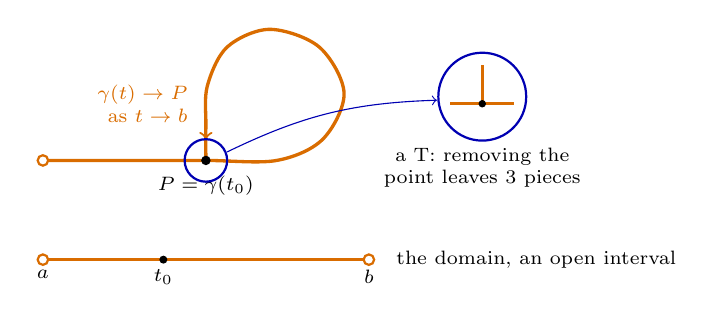
\begin{tikzpicture}[scale=0.9]
\draw[orange!85!black, very thick] plot[smooth, tension=0.55] coordinates {(-2.3,0) (-1.2,0) (0,0) (1.0,0.0) (1.65,0.3) (1.95,0.95) (1.6,1.6) (0.9,1.85) (0.3,1.6) (0.02,1.05) (0,0.5) (0,0)};
\draw[orange!85!black, fill=white, thick] (-2.3,0) circle (2.1pt);
\fill (0,0) circle (1.9pt); \node[font=\scriptsize, anchor=north] at (0,-0.08) {$P = \gamma(t_0)$};
\draw[->, orange!85!black, thick] (0,0.62) -- (0,0.3);
\node[orange!85!black, font=\scriptsize, anchor=east, align=right] at (-0.12,0.8) {$\gamma(t) \to P$\\ as $t \to b$};
\draw[blue!70!black, thick] (0,0) circle (0.3);
\draw[blue!70!black, thick] (3.90,0.90) circle (0.62);
\draw[orange!85!black, very thick] (3.45,0.80) -- (4.35,0.80); \draw[orange!85!black, very thick] (3.90,0.80) -- (3.90,1.35);
\fill (3.90,0.80) circle (1.5pt);
\draw[->, blue!70!black] (0.3,0.12) to[bend left=12] (3.26,0.85);
\node[font=\scriptsize, align=center] at (3.90,-0.10) {a T: removing the\\ point leaves 3 pieces};
\draw[orange!85!black, very thick] (-2.3,-1.4) -- (2.3,-1.4); \draw[orange!85!black, fill=white, thick] (-2.3,-1.4) circle (2.1pt) node[below, font=\scriptsize, text=black] {$a$}; \draw[orange!85!black, fill=white, thick] (2.3,-1.4) circle (2.1pt) node[below, font=\scriptsize, text=black] {$b$};
\fill (-0.6,-1.4) circle (1.6pt) node[below, font=\scriptsize] {$t_0$};
\node[font=\scriptsize, anchor=west] at (2.55,-1.4) {the domain, an open interval};
\end{tikzpicture}
